\chapter{Lichtbrechung in der Atmosph"are\label{chapter:thema}}
\lhead{Lichtbrechung in der Atmosph"are}
\begin{refsection}
\chapterauthor{Simon Sch"afer und Tibor Schneider}

\printbibliography[heading=subbibliography]
\end{refsection}

\begin{figure}
\centering
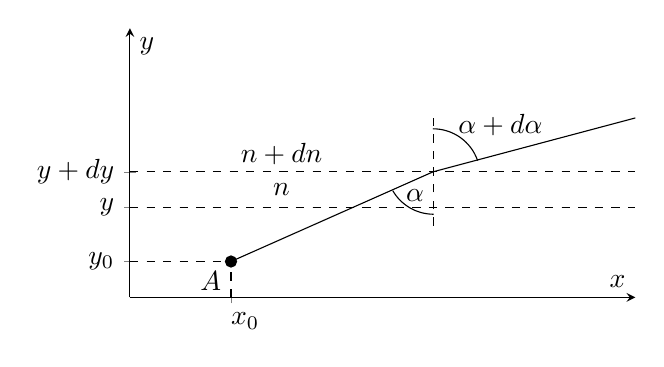
\begin{tikzpicture}
  \begin{axis}[xlabel=$x$, ylabel = $y$, axis lines=middle, height=5cm, width = 8cm,
  ymin=0, ymax=1.5, xmin=0, xmax=1, yticklabels={$y_0$, $y$, $y + dy$}, ytick =
  {0.2,0.5,0.7}, xtick={0.2}, xticklabel={\rlap{$x_0$}}]
    \draw[dashed] (axis cs:0,0.5) -- (axis cs:1,0.5);
    \draw[dashed] (axis cs:0,0.7) -- (axis cs:1,0.7);
    \draw[dashed] (axis cs:0,0.5) -- (axis cs:1,0.5);
    \draw[dashed] (axis cs:0.2,0) -- (axis cs:0.2,0.2);
    \draw[dashed] (axis cs:0,0.2) -- (axis cs:0.2,0.2);
    \filldraw (axis cs:0.2,0.2) circle (2pt) node[anchor=north east] {$A$};
    \draw (axis cs:0.2,0.2) -- (axis cs:0.6,0.7);
    \draw (axis cs:0.6,0.7) -- (axis cs:1,1);
    \draw (axis cs:0.52, 0.595) arc (210:270:0.6cm) node[anchor=north east, yshift =
    +0.44cm] {$\alpha$};
    \draw (axis cs:0.688,0.762) arc (19:90:0.6cm) node[anchor=west, yshift=+0.05cm,
    xshift=+0.2cm] {$\alpha + d\alpha$};  
    \draw[dashed](axis cs:0.6,0.4) -- (axis cs:0.6,1);
    \draw (axis cs:0.3, 0.6) node {$n$};
    \draw (axis cs:0.3, 0.8) node {$n + dn$};
  
  \end{axis}
\end{tikzpicture}
\caption{Skizze}
\label{fig:13_1}
\end{figure}


Es wird von der Snell's Gleichung ausgegangen: $n_1 \sin \alpha_1 = n_2 \sin \alpha_2$.
Durch Einsetzen der Oberen Grafik ergibt sich:

\begin{equation} \label{eq:13_1}
  n \cdot \sin(\alpha) = n_0 \cdot \sin(\alpha_0) = \varepsilon
\end{equation}

Aus der Geometrie in der Abbildung \ref{fig:13_1} ist ersichtlich:
$$\frac{\cos \alpha}{\sin \alpha} = \frac{dy}{dx} = y'(x)$$
$$\Rightarrow y'(x)^2 = \frac{1 - \sin^2 \alpha}{\sin^2 \alpha} = \frac{1}{\sin^2
\alpha} - 1$$
\begin{equation} \label{eq:13_2}
\sin^2 (\alpha) = \frac{1}{y'(x)^2 + 1}
\end{equation}

Nun quadrieren wir die Gleichung \ref{eq:13_1}, setzen \ref{eq:13_2} ein und l"osen
nach $y'(x)$ auf:
$$n^2 \cdot \frac{1}{y'(x)^2 + 1} = \varepsilon$$
\begin{equation} \label{eq:13_3}
\Rightarrow y'(x)^2 = \left( \frac{n}{\varepsilon} \right)^2 - 1
\end{equation}

In einer ersten Ann"aherung approximieren wir $n(y) = 1 + \mu e^{-\sigma y}$ und erhalten
somit die Differentialgleichung:
\begin{equation} \label{eq:13_4}
y'(x)^2 = \left( \frac{1 + \mu e^{-\sigma y}}{\varepsilon} \right)^2 - 1
\end{equation}

Nun l"osen wir die Differentialgleichung nummerisch. Dazu wurden für $\mu$ und $\sigma$
Werte eingesetzt, bei denen die Kurve gut ersichtlich ist \ref{fig:13_2}.

\begin{figure}
\centering
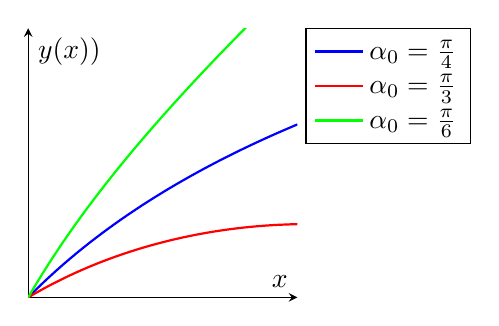
\begin{tikzpicture}
  \begin{axis}[xlabel=$x$, ylabel=$y(x))$, axis lines=middle, height=5cm, width=5cm, ticks
  = none, legend pos = outer north east, ymin = 0, ymax = 10, xmin = 0, xmax = 10] 
  \addplot [mark = none, thick, draw=blue] coordinates{
      (0.00000, 0.00000) (0.00005, 0.00005) (0.00010, 0.00010) (0.00015, 0.00015)
      (0.00020, 0.00020) (0.00044, 0.00045) (0.00069, 0.00070) (0.00094, 0.00095)
      (0.00118, 0.00121) (0.00241, 0.00246) (0.00364, 0.00372) (0.00488, 0.00497)
      (0.00611, 0.00623) (0.01226, 0.01250) (0.01842, 0.01877) (0.02457, 0.02503)
      (0.03073, 0.03128) (0.06150, 0.06249) (0.09228, 0.09357) (0.12306, 0.12453)
      (0.15383, 0.15535) (0.30772, 0.30767) (0.46160, 0.45701) (0.61549, 0.60350)
      (0.76937, 0.74724) (1.01937, 0.97516) (1.26937, 1.19649) (1.51937, 1.41160)
      (1.76937, 1.62083) (2.01937, 1.82447) (2.26937, 2.02281) (2.51937, 2.21610)
      (2.76937, 2.40458) (3.01937, 2.58847) (3.26937, 2.76797) (3.51937, 2.94328)
      (3.76937, 3.11457) (4.01937, 3.28200) (4.26937, 3.44573) (4.51937, 3.60590) 
      (4.76937, 3.76263) (5.01937, 3.91607) (5.26937, 4.06633) (5.51937, 4.21351) 
      (5.76937, 4.35773) (6.01937, 4.49908) (6.26937, 4.63766) (6.51937, 4.77354) 
      (6.76937, 4.90683) (7.01937, 5.03760) (7.26937, 5.16591) (7.51937, 5.29185) 
      (7.76937, 5.41548) (8.01937, 5.53687) (8.26937, 5.65607) (8.51937, 5.77315) 
      (8.76937, 5.88816) (9.01937, 6.00115) (9.26937, 6.11218) (9.51937, 6.22130) 
      (9.76937, 6.32854) (9.82703, 6.35302) (9.88468, 6.37739) (9.94234, 6.40168) 
      (10.00000, 6.42586)};
    \addlegendentry{$\alpha_0 = \frac{\pi}{4}$}
      
    \addplot [mark = none, thick, draw=red] coordinates{
      (0.00000, 0.00000) (0.00008, 0.00005) (0.00017, 0.00010) (0.00025, 0.00015)
      (0.00034, 0.00020) (0.00076, 0.00045) (0.00119, 0.00070) (0.00161, 0.00095) 
      (0.00203, 0.00121) (0.00415, 0.00246) (0.00627, 0.00372) (0.00838, 0.00497) 
      (0.01050, 0.00622) (0.02108, 0.01249) (0.03167, 0.01874) (0.04225, 0.02499) 
      (0.05283, 0.03122) (0.10575, 0.06225) (0.15866, 0.09302) (0.21158, 0.12355) 
      (0.26450, 0.15383) (0.51450, 0.29366) (0.76450, 0.42828) (1.01450, 0.55787) 
      (1.26450, 0.68260) (1.51450, 0.80262) (1.76450, 0.91807) (2.01450, 1.02910) 
      (2.26450, 1.13583) (2.51450, 1.23837) (2.76450, 1.33684) (3.01450, 1.43133) 
      (3.26450, 1.52194) (3.51450, 1.60876) (3.76450, 1.69187) (4.01450, 1.77134) 
      (4.26450, 1.84725) (4.51450, 1.91968) (4.76450, 1.98867) (5.01450, 2.05429) 
      (5.26450, 2.11659) (5.51450, 2.17563) (5.76450, 2.23145) (6.01450, 2.28410) 
      (6.26450, 2.33362) (6.51450, 2.38004) (6.76450, 2.42341) (7.01450, 2.46375) 
      (7.26450, 2.50109) (7.51450, 2.53547) (7.76450, 2.56690) (8.01450, 2.59541) 
      (8.26450, 2.62102) (8.51450, 2.64377) (8.76450, 2.66365) (9.01450, 2.68064) 
      (9.26450, 2.69479) (9.44837, 2.70270) (9.63225, 2.70993) (9.81612, 2.71730) 
      (10.00000, 2.72226)};
    \addlegendentry{$\alpha_0 = \frac{\pi}{3}$}
    
    \addplot [mark = none, thick, draw=green] coordinates{
      (0.00000, 0.00000) (0.00003, 0.00005) (0.00006, 0.00010) (0.00009, 0.00015)
      (0.00012, 0.00020) (0.00026, 0.00045) (0.00041, 0.00070) (0.00055, 0.00095) 
      (0.00070, 0.00121) (0.00142, 0.00246) (0.00215, 0.00372) (0.00287, 0.00497) 
      (0.00360, 0.00623) (0.00722, 0.01250) (0.01085, 0.01877) (0.01447, 0.02504) 
      (0.01810, 0.03130) (0.03623, 0.06257) (0.05435, 0.09375) (0.07248, 0.12485) 
      (0.09061, 0.15586) (0.18125, 0.30967) (0.27189, 0.46147) (0.36253, 0.61132) 
      (0.45317, 0.75931) (0.70317, 1.15839) (0.95317, 1.54514) (1.20317, 1.92073) 
      (1.45317, 2.28617) (1.70317, 2.64234) (1.95317, 2.99002) (2.20317, 3.32991) 
      (2.45317, 3.66261) (2.70317, 3.98869) (2.95317, 4.30863) (3.20317, 4.62288) 
      (3.45317, 4.93184) (3.70317, 5.23589) (3.95317, 5.53535) (4.20317, 5.83053) 
      (4.45317, 6.12171) (4.70317, 6.40914) (4.95317, 6.69305) (5.20317, 6.97367) 
      (5.45317, 7.25120) (5.70317, 7.52581) (5.95317, 7.79767) (6.20317, 8.06696) 
      (6.45317, 8.33381) (6.70317, 8.59836) (6.95317, 8.86075) (7.20317, 9.12108) 
      (7.45317, 9.37948) (7.70317, 9.63604) (7.95317, 9.89087) (8.20317, 10.14406) 
      (8.45317, 10.39568) (8.70317, 10.64583) (8.95317, 10.89458) (9.20317, 11.14200) 
      (9.45317, 11.38816) (9.58988, 11.52226) (9.72659, 11.65601) (9.86329, 11.78942) 
      (10.00000, 11.92250) };
    \addlegendentry{$\alpha_0 = \frac{\pi}{6}$} 
  \end{axis}
\end{tikzpicture}
\caption{Nummerische Lösung der Differentialgleichung (\ref{eq:13_4})}
\label{fig:13_2}
\end{figure}








